\documentclass{article}
\usepackage{listings}
\usepackage{mathrsfs}
\usepackage[utf8]{inputenc}
\usepackage{amssymb}
\usepackage{lipsum}
\usepackage{amsmath}
\usepackage{fancyhdr}
\usepackage{geometry}
\usepackage{scrextend}
\usepackage[english,german]{babel}
\usepackage{titling}
\setlength{\droptitle}{-3cm}
\usepackage{tikz}
\usepackage{algorithm,algpseudocode}
\usepackage[doublespacing]{setspace}
\usetikzlibrary{datavisualization}
\usetikzlibrary{datavisualization.formats.functions}
\usepackage{polynom}
\usepackage{amsmath}
\usepackage{gauss}
\usepackage{tkz-euclide}
\usetikzlibrary{datavisualization}
\usetikzlibrary{datavisualization.formats.functions}
\author{
Alexander Mattick Kennung: qi69dube\\
Kapitel 1
}
\usepackage{import}
\date{\today}
\geometry{a4paper, margin=2cm}
\usepackage{stackengine}
\parskip 1em
\newcommand\stackequal[2]{%
  \mathrel{\stackunder[2pt]{\stackon[4pt]{=}{$\scriptscriptstyle#1$}}{%
  $\scriptscriptstyle#2$}}
 }
\makeatletter
\renewcommand*\env@matrix[1][*\c@MaxMatrixCols c]{%
  \hskip -\arraycolsep
  \let\@ifnextchar\new@ifnextchar
  \array{#1}}
\makeatother
\lstset{
  language=haskell,
}
\lstnewenvironment{code}{\lstset{language=Haskell,basicstyle=\small}}{}
\usepackage{enumitem}
\setlist{nosep}
\usepackage{titlesec}

\titlespacing*{\subsection}{0pt}{2pt}{3pt}
\titlespacing*{\section}{0pt}{0pt}{5pt}
\titlespacing*{\subsubsection}{0pt}{1pt}{2pt}
\title{Vorlesung 4}


\begin{document}
	\maketitle
	\section{Präsenz 39}
	A = ``Zwei geräte pro Stunde''\\
	Schlüsselwörter: ``Stetig gleichverteilt''.\\
	a)\\
	Unabhängig.\\
	\[f(x) = \begin{cases}\frac{1}{b-a}&a<x<n\\ 0&sonst\end{cases}\]
	stetig gleichverteilt.\\
	$x_i$ die Reparaturdauer in Minuten für $i\in\{1,2\}$\\
	\[f_i(x_i)= \begin{cases}\frac{1}{40-10}&10<x<40\\ 0&sonst\end{cases}\]
	Wenn beide Zeiten unabhänig sind, zwei Erfolge.\\
	\[f(x_1,x_2) =  \begin{cases}\frac{1}{30}\cdot \frac{1}{30}&10<x_1<40\land 10<x_2<40\\ 0&sonst\end{cases}\]
	\[P(x_1+x_2\leq 60)=\]
	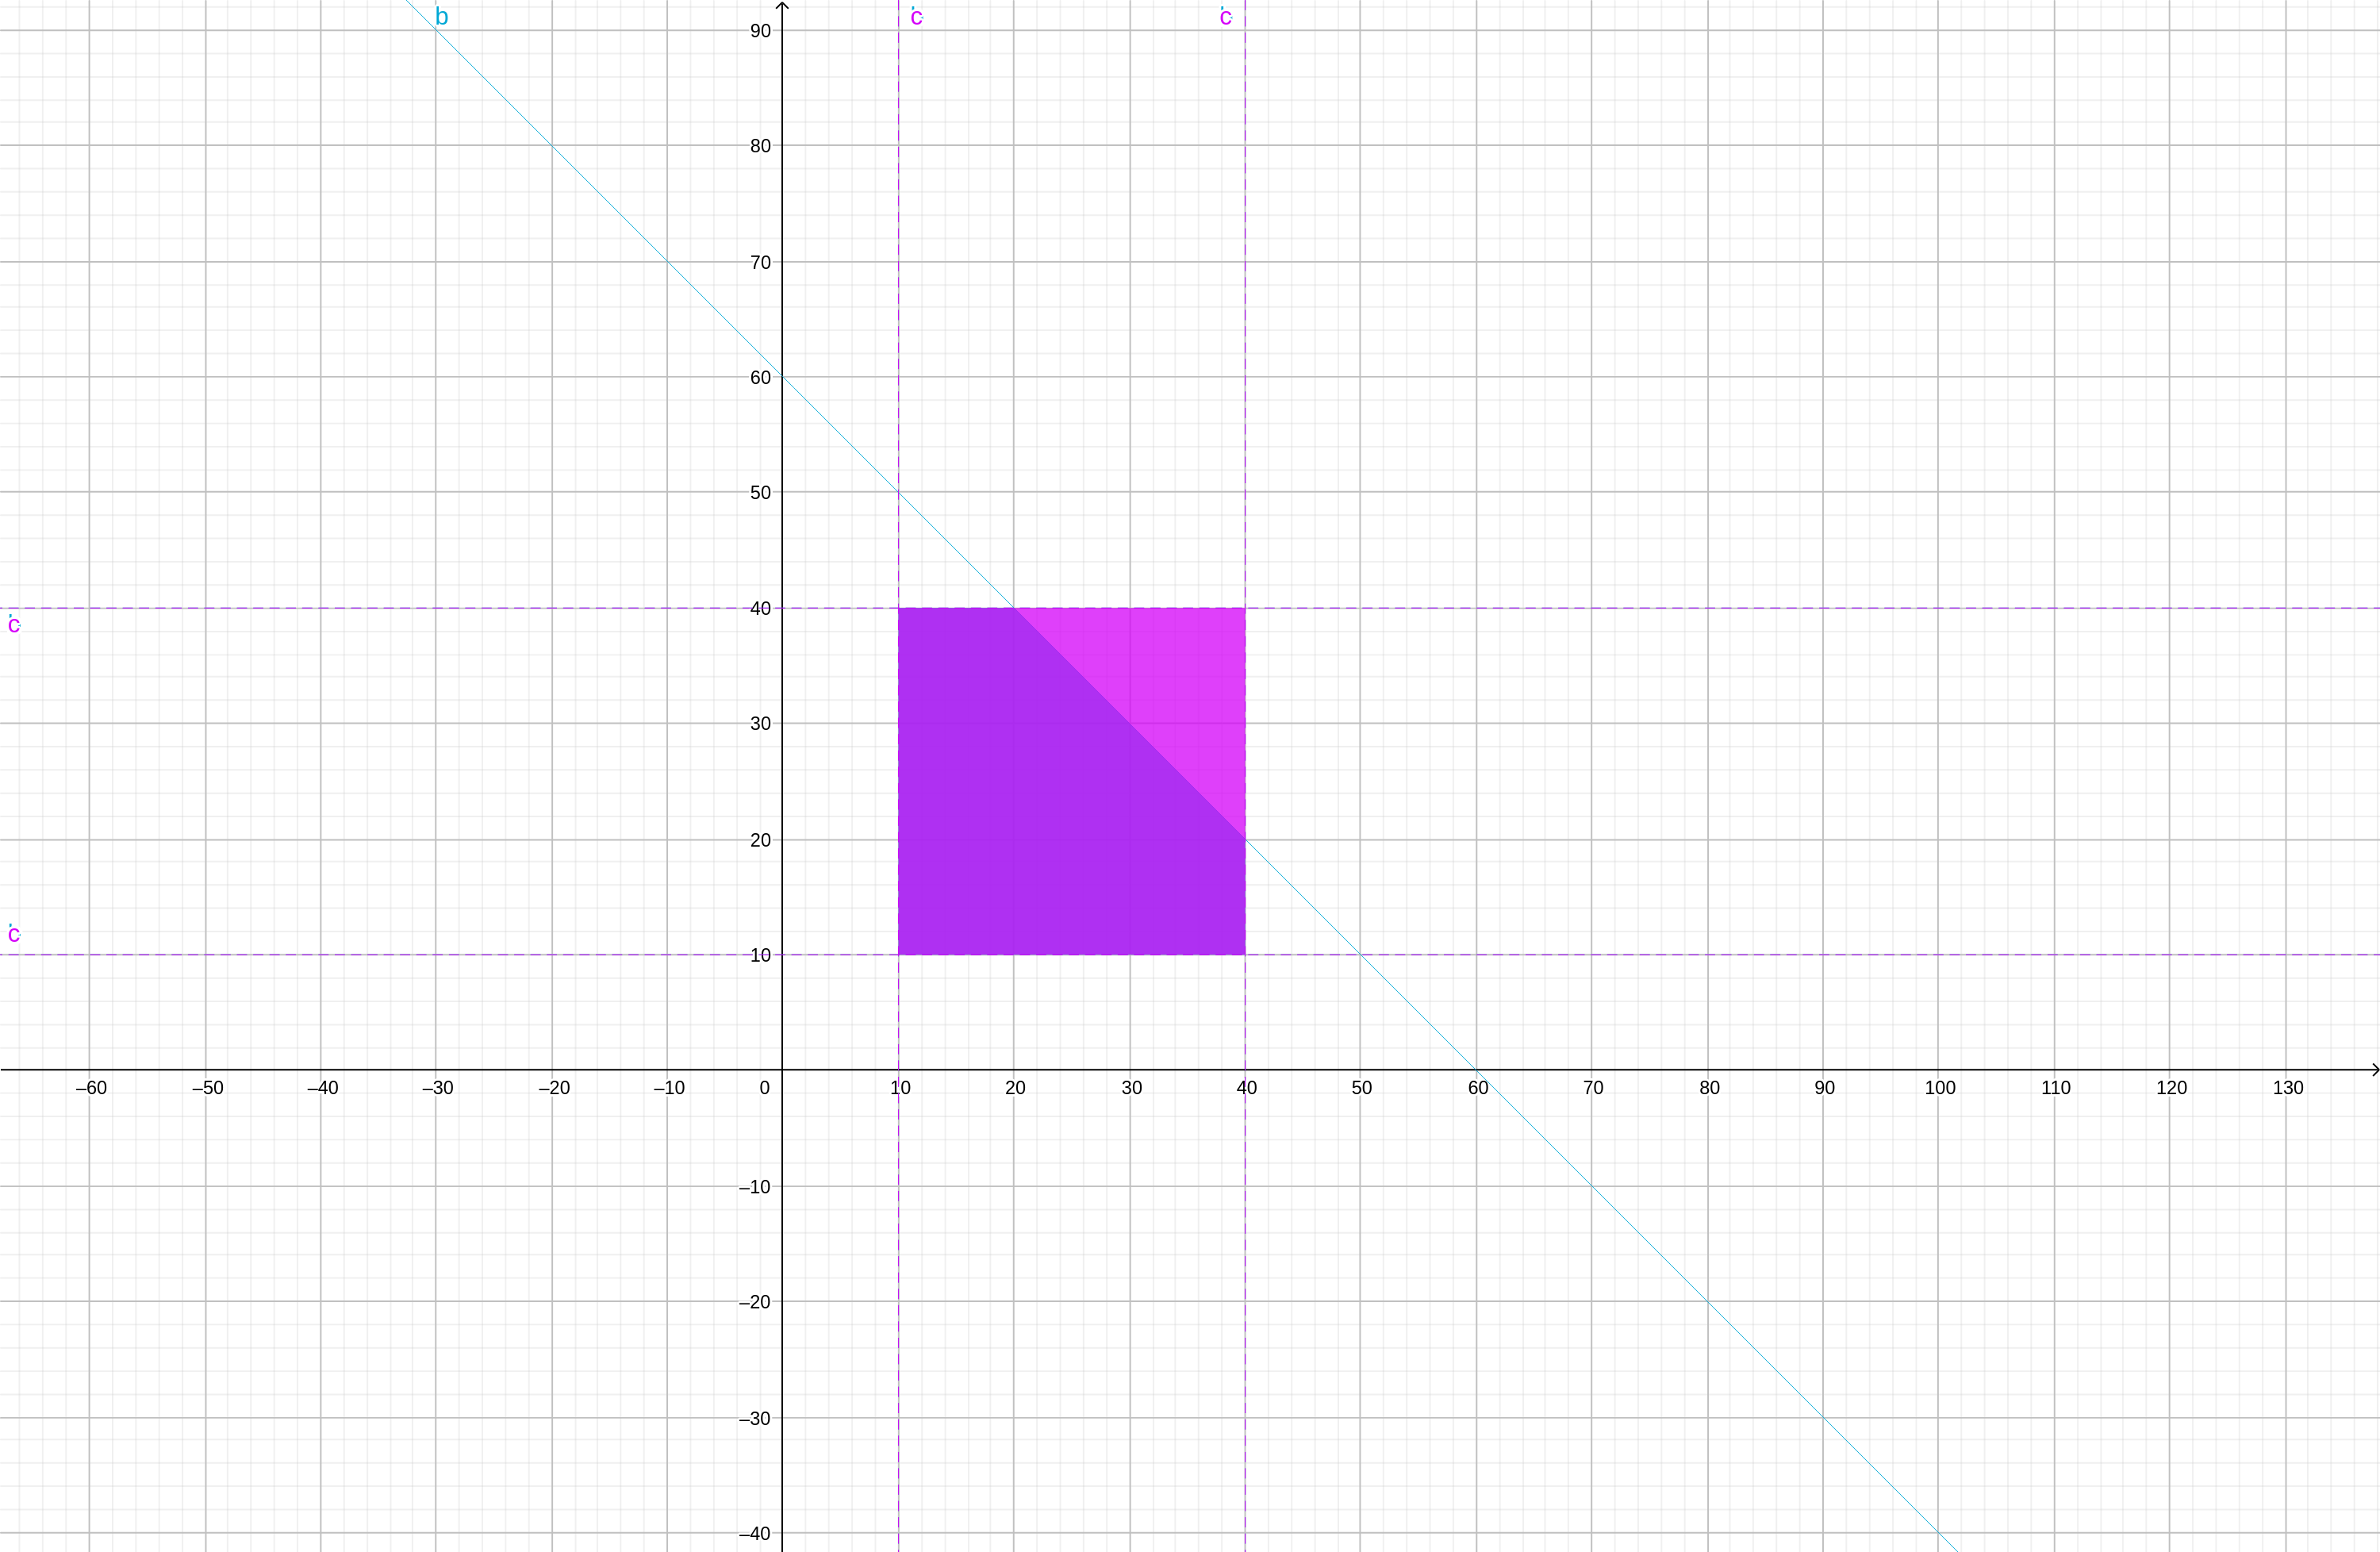
\includegraphics[height=256px]{SkizzePräsenz.png}\\
	$$\int\int_{x_1+x_2\leq 60}f(x_1,x_2)dx_1dx_2$$
	$$\int\int_{x_1+x_2\leq 60}\frac{1}{900}dx_1dx_2$$
	Integral über die Fläche von A mal $\frac{1}{900}$.\\
	b)\\
	\[f(x_1)=\begin{cases}\frac{1}{30}&10<x_1<40\\ 0&sonst\end{cases}\]
	\[f(x_2;x_1) = \begin{cases}\frac{1}{30}&10<x_1<30\land 20<x_2<50 \\\frac{1}{30}& 30<x_1<40\land 10<x_2\leq 40 \\0&sonst\end{cases} \]
	Beim ersten fall hat man die 10 minuten Pause vor $x_2$
	\[f(x_1,x_2) = f(x_1)f(x_2;x_1) =\begin{cases}\frac{1}{900}&10<x_1<30\land 20<x_2<50 \\\frac{1}{900}& 30<x_1<40\land 10<x_2\leq 40 \\0&sonst\end{cases}\]
	\[P(x_1+x_2\leq 60) = \int\int_{x_1+x_2\leq 60}f(x_1,x_2) dx_1dx_2\]
	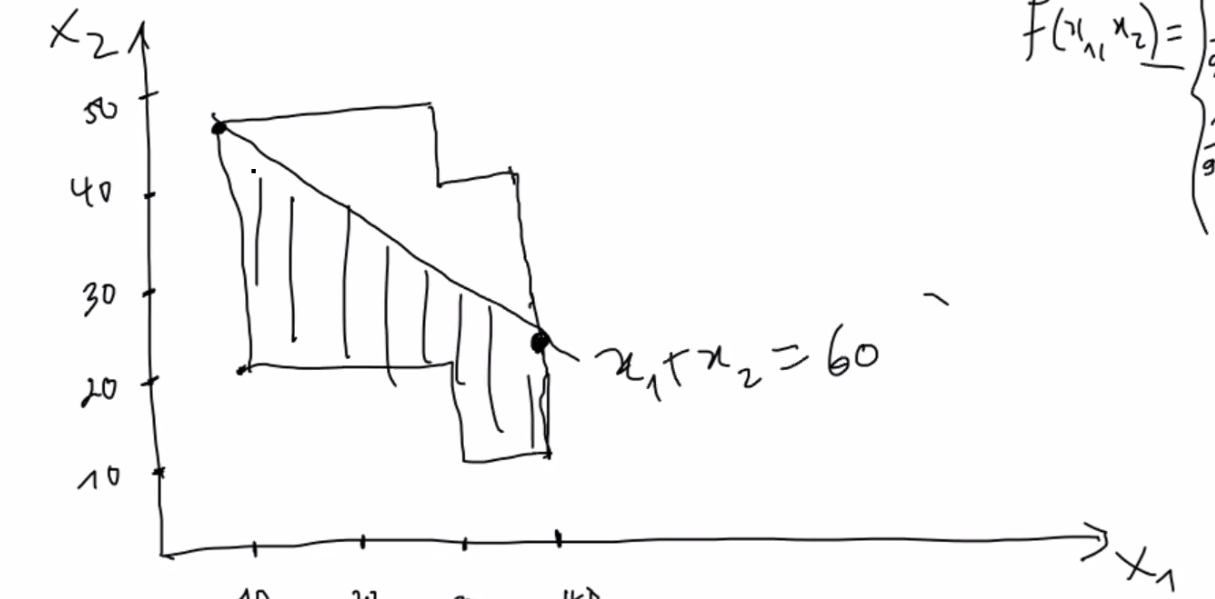
\includegraphics[height=256px]{Skizze2.png}\\
	\[P(x_1+x_2\leq 60) = |A|\frac{1}{900}\]
	b)\\
	$\Omega_i =\{R,F\}$ R nicht fehlgeleitet. F= Fehlgeleitet.\\
	Für $i\in\{1,2,3\}$ $\Omega=\Omega_i^3$ und $\mathscr{A}=P(\Omega)$.\\
	\[P(\{\omega\})=P(\omega_1,\omega_2,\omega_3) = f_1(\omega_1)f^1_2(\omega_2;\omega_1)f^2_3(\omega_3;\omega_1,\omega_2)\]
	$f_1(R)=1-p, f_1(F)=P$\\
	$f_2^1(F;F) = 1,f_2^1(R;F)=0, f_2^1(F;R) = p, f_2^1(R;R) = 1-p$\\
	$f_3^2(F;F,F) = 1,f_3^2(R;F,F)=0, f_3^2(R;R,R) = p^3, f_3^2(F;R,R)= p$\\
	A = irgendwo fehlgeleitet $\{\omega\in \Omega| \omega_3 =F\}$\\
	B = An i-ter stelle fehlgeleitet $\{\omega\in \Omega| \omega_i =F\land \omega_j= R\forall j<i\}$\\
	$P(B_i|A) = \frac{P(B_i\cap A)}{P(A)}$\\
	\[P(A) = 1-P(A^c) = 1-P(\{\omega\in\Omega|\omega_3=R\}) = 1-\sum_{\omega_i\in\Omega_i}f_1(R)f^1_2(\omega_2; \omega_1)f^2_3(\omega_3; \omega_1,\omega_2) = 1- (1-p)(1-p)(1-p) = 1-(1-p)^3\]
	\[B_i = \{\omega\in\Omega|\omega_i = F\land \omega_j=R\forall j<i\}\]
	$B_1 =\{F\}\times \Omega_2\times \Omega_3\implies B_1\cap A =\{(F,R,F), (F,F,F)\}$\\
	$B_2 \implies A\cap B_2 = \{(R,F,R),(R,F,F)\}$\\
	$B_3\subset A \implies B_3\cap A = B_3$\\
	$p(B_1\cap A) = P$\\
	$p(B_2\cap A) = P(1-P)$\\
	$p(B_3\cap A) = P(1-P)^2$\\



\end{document}
